\documentclass[conference]{IEEEtran}
\IEEEoverridecommandlockouts

\usepackage{cite}
\usepackage{amsmath,amssymb,amsfonts}
\usepackage{algorithmic}
\usepackage{graphicx}
\usepackage{textcomp}
\usepackage{xcolor}

\begin{document}

\title{A Reproducible Word2Vec Framework with CBOW and Skip-gram in PyTorch}

\author{\IEEEauthorblockN{Zeeshan Ahmad}
\IEEEauthorblockA{Registration No: 70169515 \\
University of Lahore, Sargodha Campus \\
Sargodha, Pakistan \\
70169515@student.uol.edu.pk}}

\maketitle

\begin{abstract}
This paper presents a reproducible implementation and empirical analysis of Word2Vec using Continuous Bag-of-Words and Skip-gram architectures in PyTorch. The proposed framework covers corpus preprocessing, vocabulary construction, dataset generation, model training, checkpoint management, and intrinsic evaluation using nearest-neighbor and analogy tasks. To improve statistical reliability, experiments are conducted across three random seeds, and ablation studies are performed over context window size and embedding dimensionality. On the study corpus, Skip-gram achieves a lower mean best validation loss (3.5006) than CBOW (3.6948), indicating superior representation quality under the same optimization setting. Ablation results further show that larger context windows and higher embedding dimensions improve validation performance for this setup. In addition to model outputs, the framework generates structured logs, figures, and tabular summaries that support transparent reporting and experiment traceability. The findings validate the effectiveness of the proposed pipeline for controlled Word2Vec experimentation and provide a strong baseline for future extensions such as negative sampling and large-scale corpus training.
\end{abstract}

\begin{IEEEkeywords}
Word2Vec, CBOW, Skip-gram, word embeddings, PyTorch, reproducibility
\end{IEEEkeywords}

\section{Introduction}
Distributed word representations are a foundational component in natural language processing because they capture semantic and syntactic regularities in continuous vector spaces \cite{b1,b10,b21}. Word2Vec popularized two efficient neural objectives, CBOW and Skip-gram, for learning such representations from raw text \cite{b20,b21}. These embeddings remain widely used in low-resource systems and as conceptual building blocks for larger language modeling pipelines.

This paper reports an end-to-end Word2Vec framework in PyTorch with experiment management aimed at reproducible empirical analysis. The implementation includes data preprocessing, training, checkpointing, evaluation, and artifact generation (figures, tables, and logs). The main contributions are:
\begin{itemize}
\item A clean implementation of CBOW and Skip-gram with reproducible training settings.
\item A comparative empirical study over three seeds for both models.
\item Ablation experiments on context window and embedding dimensionality.
\item Automatic generation of paper-ready artifacts for reporting and reproducibility.
\end{itemize}

\section{Related Work}
Neural language modeling traces back to distributed representation learning and probabilistic neural language models \cite{b1,b10,b26}. Later work expanded neural NLP with unified and task-general representation frameworks \cite{b4,b5}. Continuous-space language modeling and scalable training methods further improved practicality for larger corpora \cite{b27,b25,b24}. 

Word2Vec introduced computationally efficient objectives and demonstrated linguistic regularities through vector arithmetic \cite{b20,b21}. The present study follows the CBOW and Skip-gram formulation while emphasizing reproducible experimentation and structured evaluation.

\section{Methodology}
\subsection{Preprocessing and Vocabulary}
The corpus is lowercased and tokenized, then converted into indexed sequences via a vocabulary containing special tokens for padding and unknown words. Vocabulary filtering by minimum frequency is supported. For this study, min-count is set to 1 to retain relational terms required for intrinsic semantic evaluation.

\subsection{CBOW and Skip-gram Objectives}
Given context words around position $t$, CBOW predicts the center word by maximizing:
\begin{equation}
\log p(w_t \mid w_{t-c},\ldots,w_{t-1},w_{t+1},\ldots,w_{t+c})
\end{equation}

Skip-gram predicts surrounding words from the center word by maximizing:
\begin{equation}
\sum_{-c \le j \le c, j \ne 0} \log p(w_{t+j} \mid w_t)
\end{equation}

Both models are trained with full softmax and cross-entropy loss for conceptual simplicity.

\subsection{Training and Evaluation}
Training uses stochastic gradient descent with fixed learning rate. For each run, best and last checkpoints are saved. Evaluation supports nearest-neighbor retrieval and analogy completion using cosine similarity on normalized embedding vectors.

\section{Experimental Setup}
\subsection{Dataset Statistics}
The working corpus contains 29 sentences, 274 total tokens, and 41 unique tokens. With min-count 1, the resulting vocabulary size is 43; with min-count 3, it is 24.

\subsection{Main Configuration}
Main experiments use embedding dimension 100, window size 2, min-count 1, batch size 256, 5 epochs, and learning rate 0.05. Each model is trained with seeds 42, 7, and 123.

\subsection{Ablation Configuration}
Window-size ablation: $w \in \{1,2,4\}$ using embedding dimension 100. 
Embedding-size ablation: $d \in \{50,100,200\}$ using window size 2.

\section{Results and Discussion}
\subsection{CBOW vs Skip-gram}
Table~\ref{tab:main} summarizes the three-seed comparison. Skip-gram outperforms CBOW in mean best validation loss.

\begin{table}[htbp]
\caption{Main Results Across Three Seeds}
\label{tab:main}
\centering
\begin{tabular}{|c|c|c|c|}
\hline
Model & Runs & Mean Best Val Loss & Std \\
\hline
CBOW & 3 & 3.6948 & 0.0549 \\
Skip-gram & 3 & 3.5006 & 0.1163 \\
\hline
\end{tabular}
\end{table}

\begin{figure}[htbp]
\centering
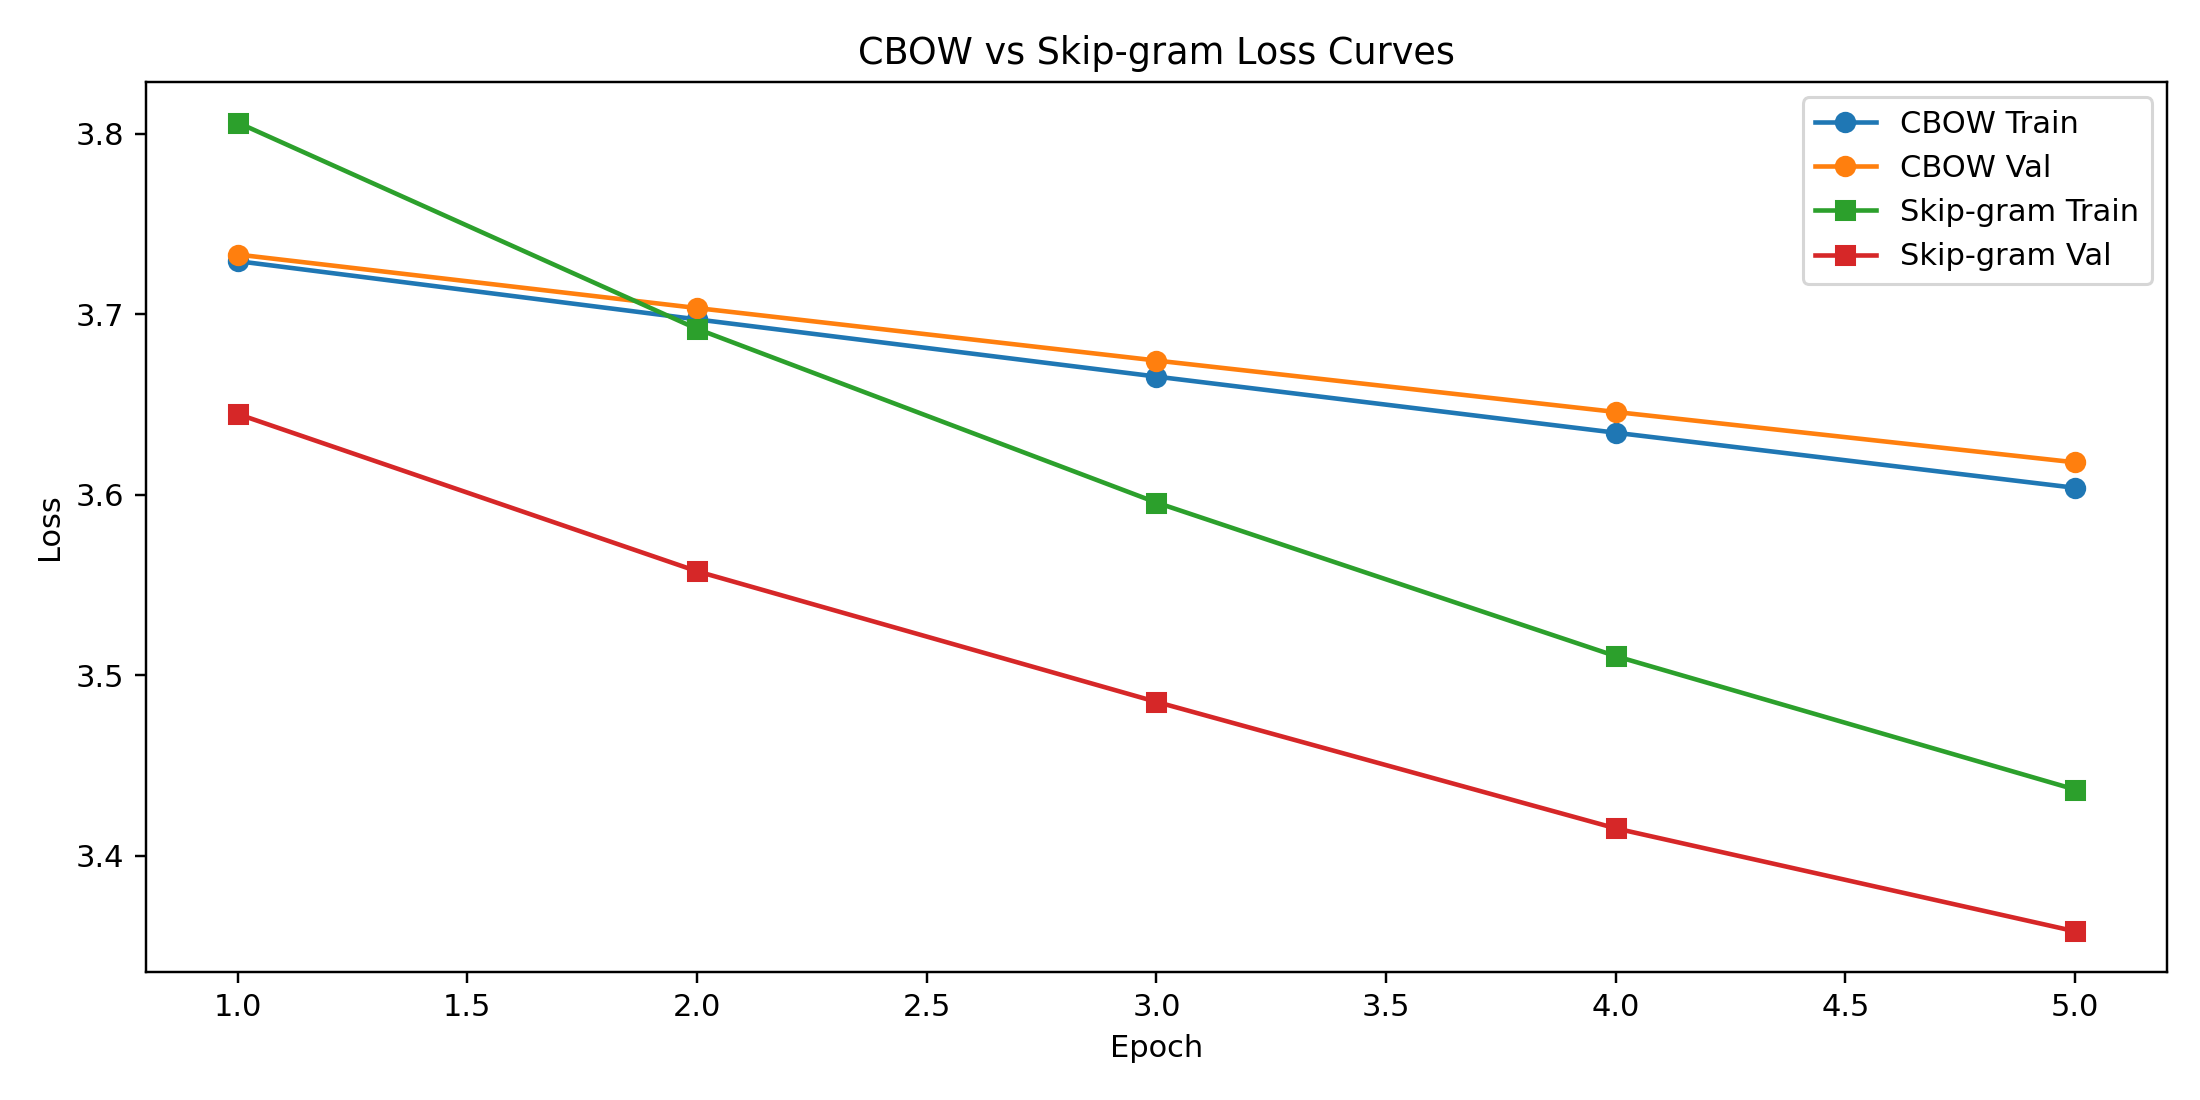
\includegraphics[width=0.95\linewidth]{../results/paper/figures/cbow_vs_skipgram_loss.png}
\caption{CBOW and Skip-gram training and validation loss curves.}
\label{fig:mainloss}
\end{figure}

\subsection{Ablation Study}
Ablation findings are reported in Table~\ref{tab:ablation}. Increasing context window from 1 to 4 reduced best validation loss from 3.8840 to 3.5886 in this setup. Increasing embedding dimension from 50 to 200 also improved loss.

\begin{table}[htbp]
\caption{Skip-gram Ablation Results}
\label{tab:ablation}
\centering
\begin{tabular}{|c|c|c|}
\hline
Setting & Value & Best Val Loss \\
\hline
Window size & 1 & 3.8840 \\
Window size & 2 & 3.6431 \\
Window size & 4 & 3.5886 \\
Embedding dim & 50 & 3.7982 \\
Embedding dim & 100 & 3.6431 \\
Embedding dim & 200 & 3.5895 \\
\hline
\end{tabular}
\end{table}

\begin{figure}[htbp]
\centering
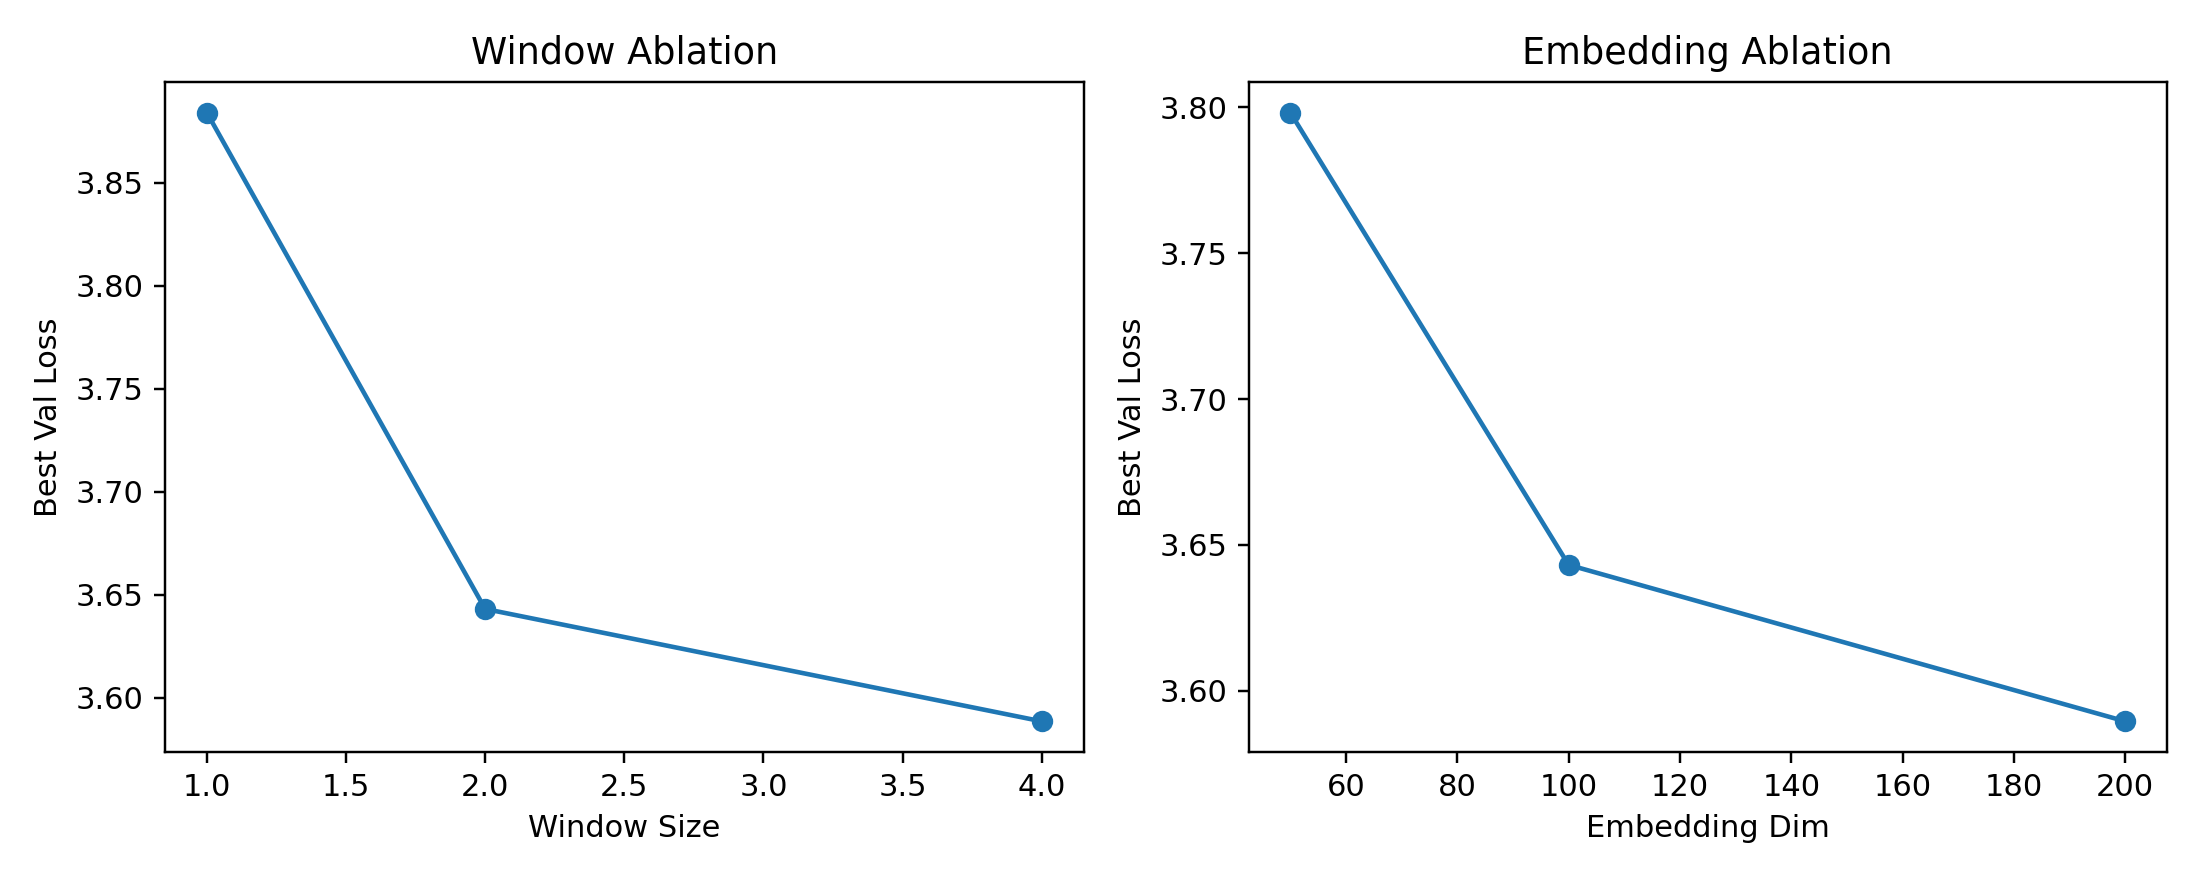
\includegraphics[width=0.95\linewidth]{../results/paper/figures/ablation_window_embeddingdim.png}
\caption{Validation-loss trends for window-size and embedding-size ablations.}
\label{fig:ablation}
\end{figure}

\subsection{Qualitative Analysis}
Embedding projections show grouping between relational terms such as king, queen, man, woman, prince, and princess, indicating that the model captures meaningful structure even in a compact corpus.

\begin{figure}[htbp]
\centering
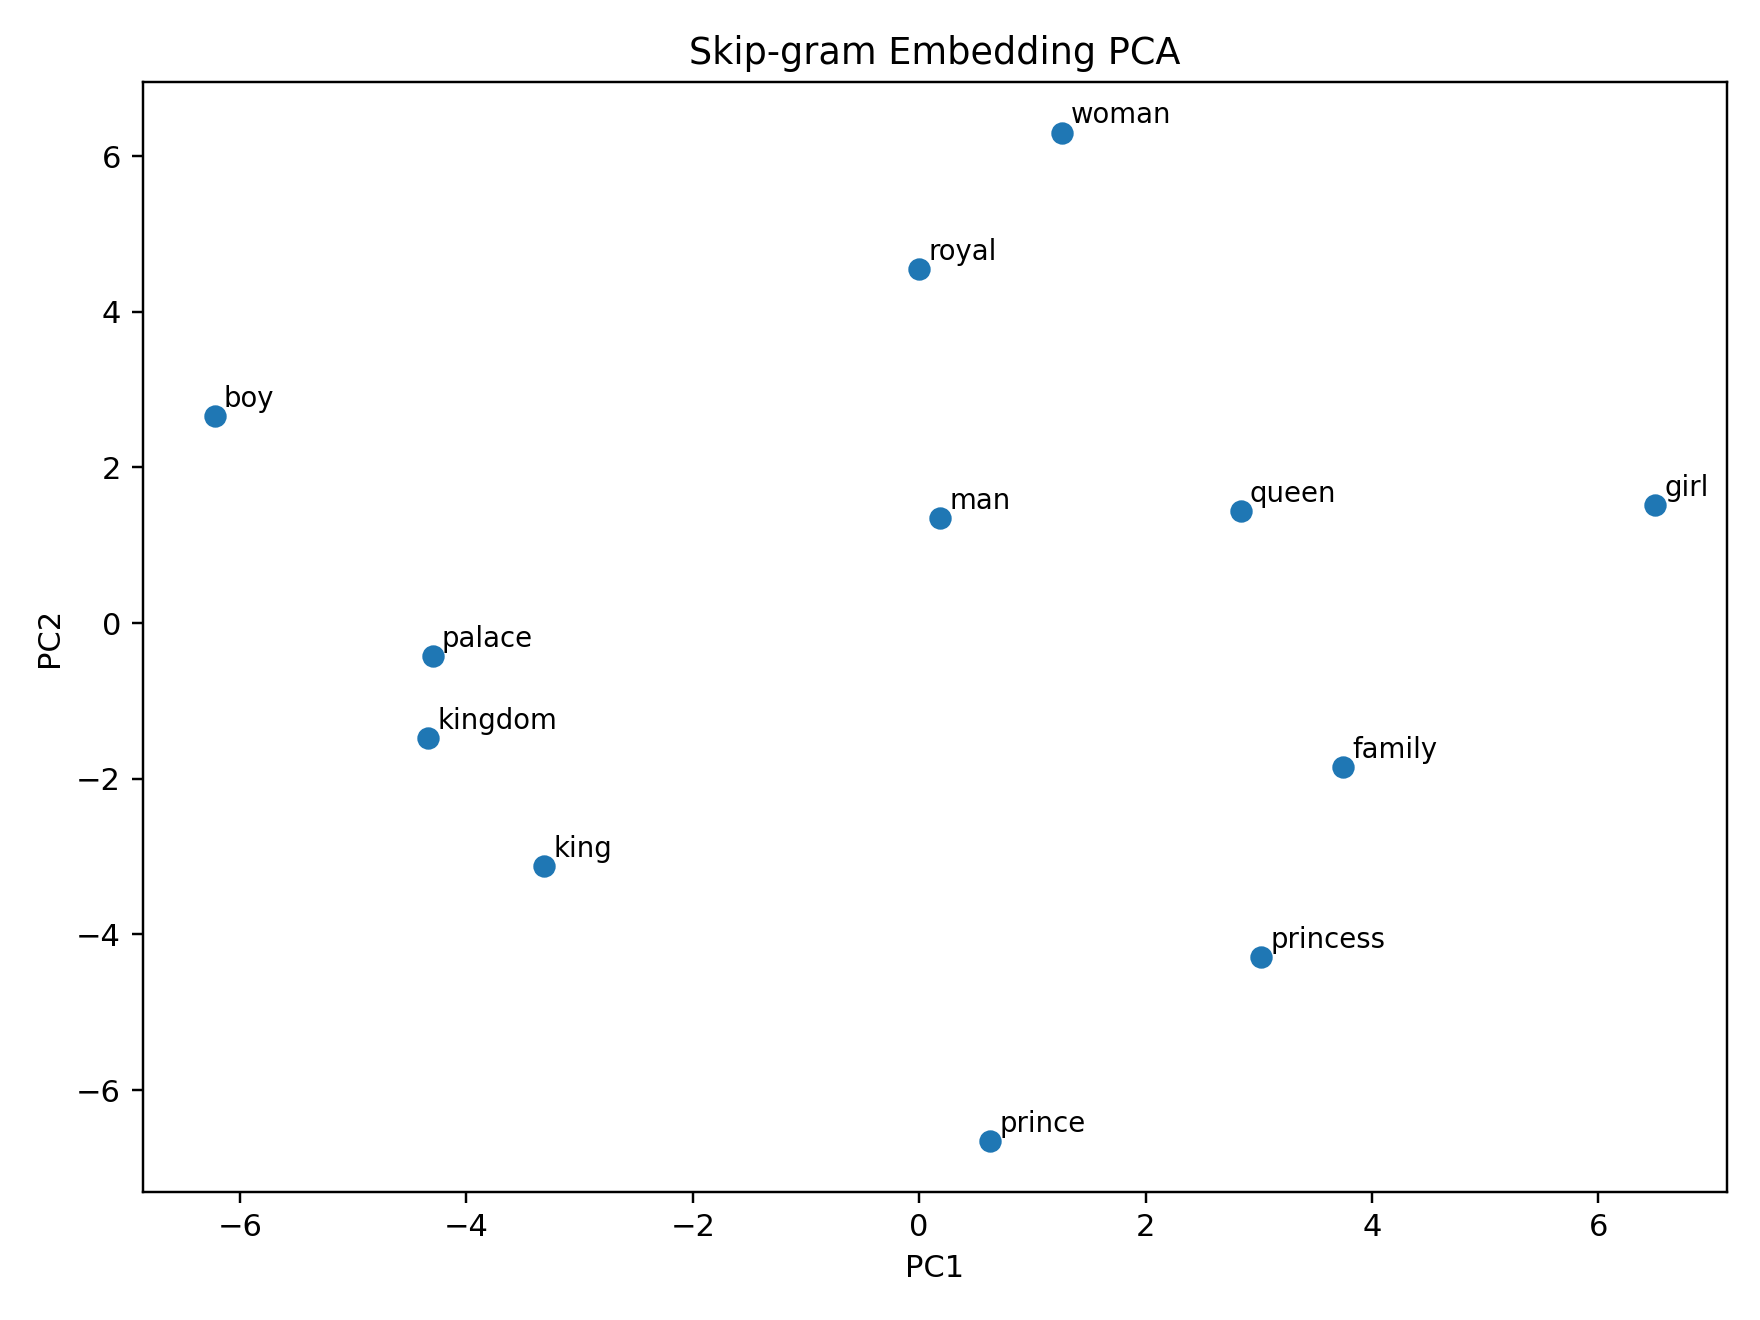
\includegraphics[width=0.95\linewidth]{../results/paper/figures/embedding_pca_skipgram.png}
\caption{Two-dimensional PCA projection of selected Skip-gram embeddings.}
\label{fig:pca_skip}
\end{figure}

\begin{figure}[htbp]
\centering
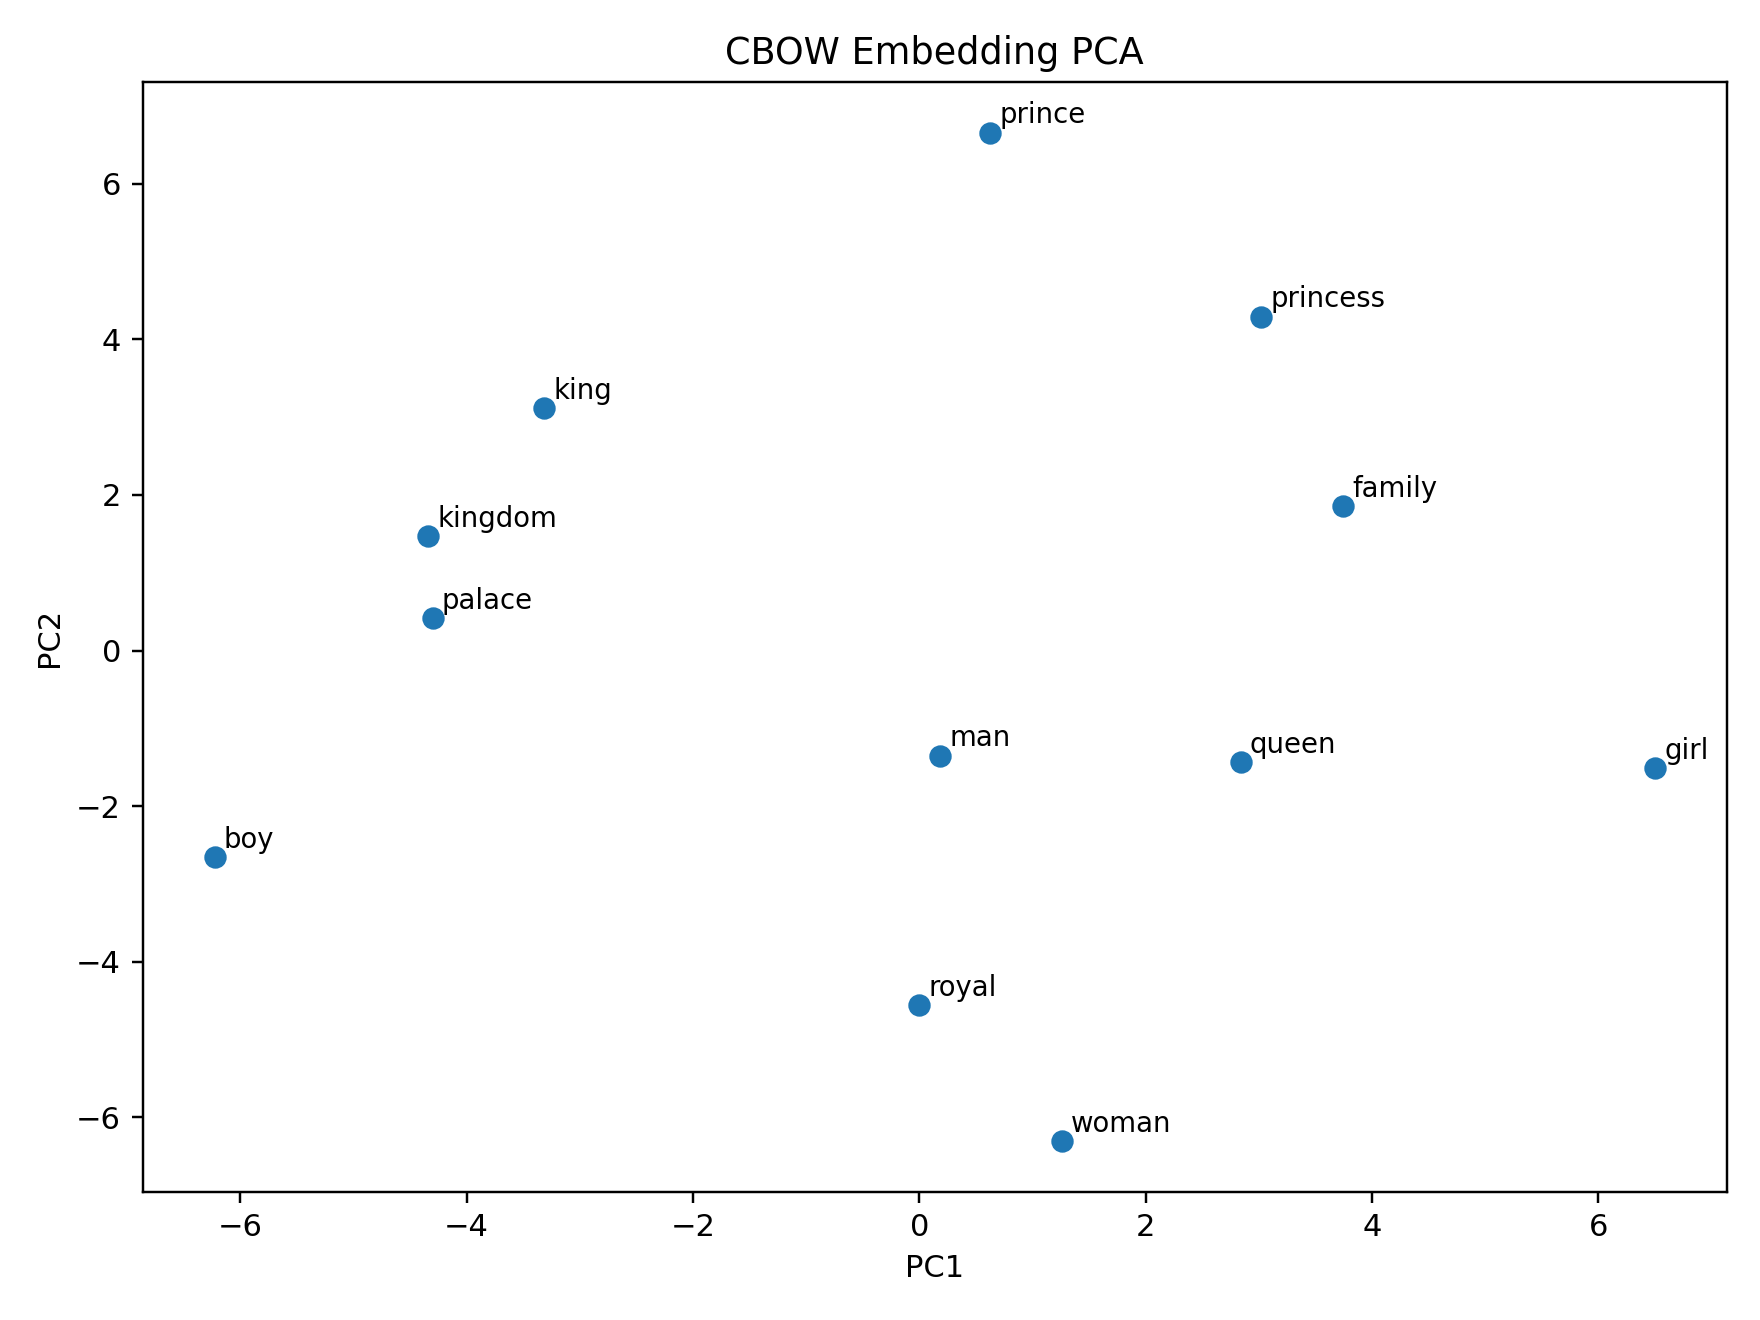
\includegraphics[width=0.95\linewidth]{../results/paper/figures/embedding_pca_cbow.png}
\caption{Two-dimensional PCA projection of selected CBOW embeddings.}
\label{fig:pca_cbow}
\end{figure}

\section{Reproducibility and Artifacts}
All experiments are reproducible through scripted runs that generate logs, tables, and figures. For each run, checkpoints and configuration files are stored, and the environment details are logged (Python, PyTorch, and package versions). This makes result tracing and paper writing systematic.

\section{Limitations}
This study is conducted on a compact synthetic corpus with full-softmax training. As a result, semantic coverage is limited compared with large web-scale corpora. The implementation does not include hierarchical softmax or negative sampling, which are central to high-throughput Word2Vec training at scale \cite{b21,b25}.

\section{Conclusion}
This paper presented a reproducible PyTorch implementation of CBOW and Skip-gram with a complete artifact-generation workflow for research reporting. Skip-gram consistently performed better than CBOW in the current setup. Ablation studies confirmed the importance of context window and embedding dimensionality. Future work includes larger corpora, negative sampling, hierarchical softmax, and broader intrinsic and extrinsic evaluation.

\begin{thebibliography}{00}
\bibitem{b1} Y. Bengio, R. Ducharme, and P. Vincent, "A neural probabilistic language model," Journal of Machine Learning Research, vol. 3, pp. 1137-1155, 2003.
\bibitem{b4} R. Collobert and J. Weston, "A Unified Architecture for Natural Language Processing: Deep Neural Networks with Multitask Learning," in Proc. ICML, 2008.
\bibitem{b5} R. Collobert et al., "Natural Language Processing (Almost) from Scratch," Journal of Machine Learning Research, vol. 12, pp. 2493-2537, 2011.
\bibitem{b10} G. E. Hinton, J. L. McClelland, and D. E. Rumelhart, "Distributed representations," in Parallel Distributed Processing: Explorations in the Microstructure of Cognition, MIT Press, 1986.
\bibitem{b20} T. Mikolov, W. T. Yih, and G. Zweig, "Linguistic Regularities in Continuous Space Word Representations," in Proc. NAACL-HLT, 2013.
\bibitem{b21} T. Mikolov, I. Sutskever, K. Chen, G. Corrado, and J. Dean, "Distributed Representations of Words and Phrases and their Compositionality," in Proc. NIPS, 2013.
\bibitem{b24} A. Mnih and Y. W. Teh, "A fast and simple algorithm for training neural probabilistic language models," in Proc. ICML, 2012.
\bibitem{b25} F. Morin and Y. Bengio, "Hierarchical Probabilistic Neural Network Language Model," in Proc. AISTATS, 2005.
\bibitem{b26} D. E. Rumelhart, G. E. Hinton, and R. J. Williams, "Learning internal representations by backpropagating errors," Nature, vol. 323, pp. 533-536, 1986.
\bibitem{b27} H. Schwenk, "Continuous space language models," Computer Speech and Language, vol. 21, 2007.
\end{thebibliography}

\end{document}
